

%\subsection{Design and Implementation Notes}

Regrid has been designed to be as efficient as possible during its
Run routine.  Although the initial calculation during the Store routines
can be computationally intensive, the {\tt ESMF\_RouteHandle} object
it creates is designed to be reused by similar Fields on the same Grids.
And, as long as the Grids are static, RegridStore can be called once
and reused throughout a simulation.  It leverages internal structures
and methods used throughout ESMF for communication so that algorithmic
and programming improvements can be focused on a single location.

Because many methods are supported for regridding, the main Store function
branches to a specific creation function based on the regrid method requested
(e.g. bilinear, conservative, spectral).  Each of these regrid methods are in
a separate module to prevent the main Regrid module from becoming too
large.  The user is unaware of this hierarchy as the top-level module provides
a unified API.

The RouteHandle object created by the RegridStore function contains a set of
"links" which identify how a Field at a point on the destination Grid is
related to a Field at a point on the source Grid.  As such, a "link"
consists of a source address, a destination address and a weight.  The addresses
are stored as indices to allow reuse by different Fields on the same Grids.
Because the Grids are generally distributed very differently, the Regrid object
also contains communication information for data motion required for the
regridding.

Our early application codes use static computational meshes, so initial 
optimization efforts have been focused on making the Regrid run routines 
fast, at the expense of the Store routines if necessary.  Therefore, Regrid
has been designed to move as much work as possible to the calculation of weights
that takes place inside Store.  In initial timings, typical RegridStore calls
take on the order of seconds while the application routines themselves require
more on the order of milliseconds.  Scaling on parallel architectures is
reasonably good up until communication overhead dominates timings (see 
Figure \ref{fig:RegridScaling} for scaling curves from an example application).

\begin{center}
\begin{figure}
\caption{Sample scaling graphs for Regrid Run and Store routines. }
\label{fig:RegridScaling}
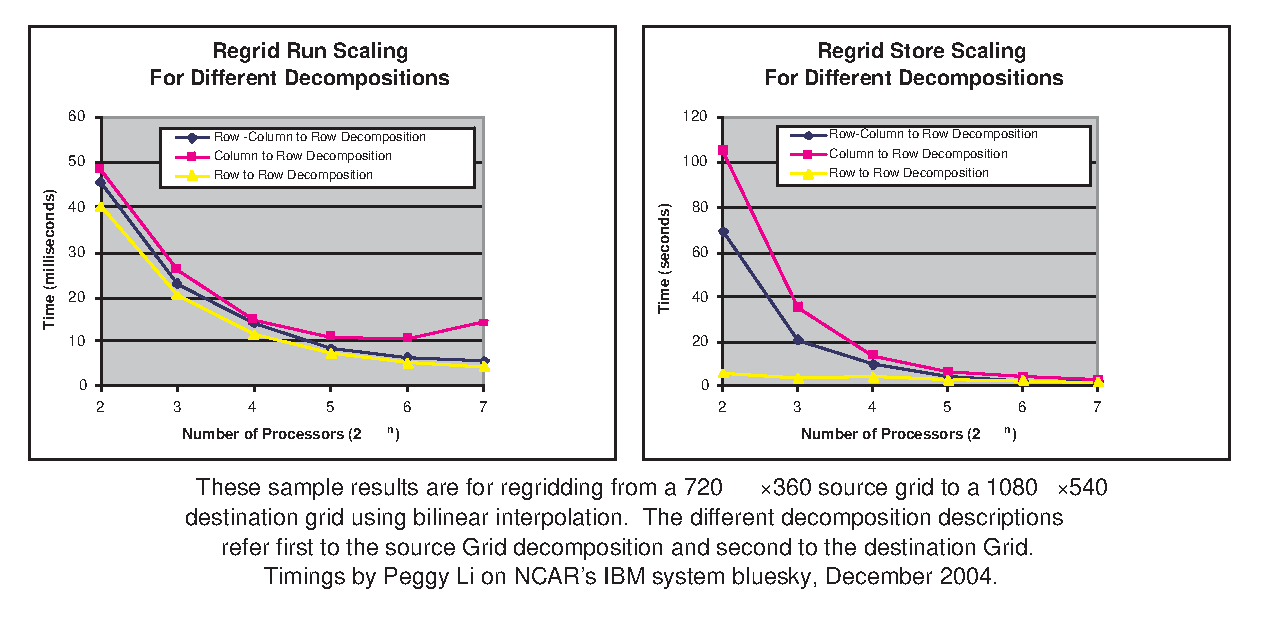
\includegraphics{RegridScaling2002}
\end{figure}
\end{center}



\subsubsection{Overview of Parallelization of Regrid}
On parallel processing platforms, the physical domains of the source and
destination Grids are decomposed into logical Decomposition Elements (DEs), as
illustrated in Figure \ref{fig:ParallelRegridding}.  In order to calculate
interpolation weights, each

\begin{center}
\begin{figure}
\caption{Illustration of Parallel Regridding. }
\label{fig:ParallelRegridding}
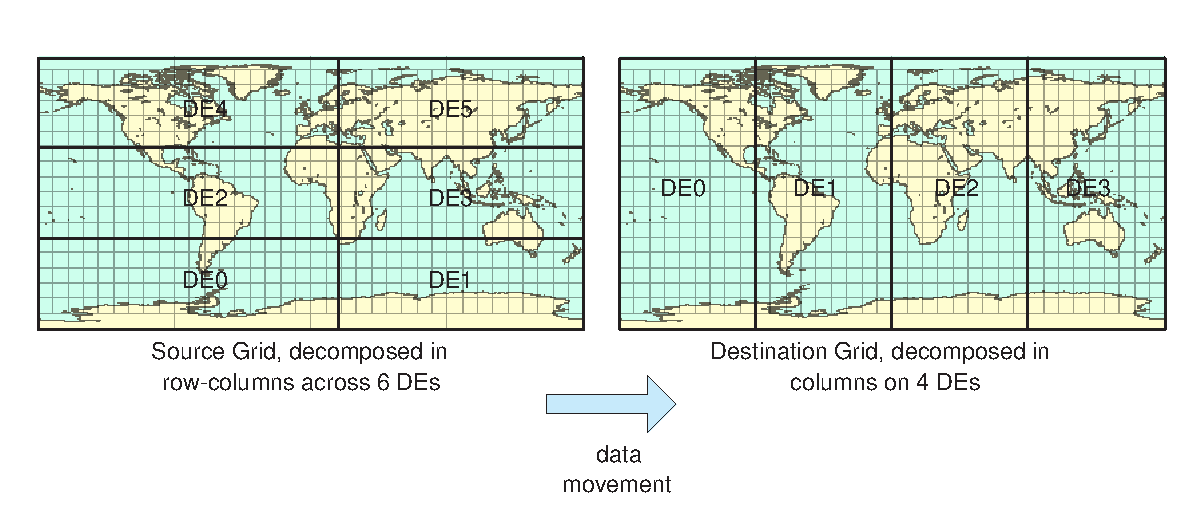
\includegraphics{ParallelRegridding2002}
\end{figure}
\end{center}

destination DE will require coordinate data from any of the source Grid that
overlaps it in physical space, which may span several DEs from the source Grid.
Corresponding source Field data is necessary later for regridding calculations
using the regridding weights.  The DEs for each Grid are mapped to sets of PETs,
which can be either shared or unique.  However, RegridStore and RegridRun must
be called with a VM encompassing the union of the sets of PETS, typically from
a CouplerComponent.  In any case, most situations will require data transfer
between PETs for regridding.  Once source data is available locally, the
regridding algorithms discussed earlier can be applied.

There are four major sections of regridding that are impacted by the
parallelization process: identifying necessary data, transferring that data, the
sweep algorithms, and then calculating and applying the interpolation weights to
calculate regridded Fields.  Each will be discussed below.


\subsubsection{Parallelization of Regrid: Identification of Necessary Data}
The calculation of interpolation weights requires coordinate information from
both source and destination Grids, and the application of those weights to
determine regridded values needs corresponding source data.  In a serial
implementation of regridding, the complete source and destination Grids, with
all their related data, are stored on a single processor.  In a parallel
implementation, the Grids and their corresponding data have been decomposed as
DEs on a number of PETs.  In this situation, none of the PETs responsible for
part of the destination Grid, represented as a DE, necessarily has all the source
data needed for the calculation or application of interpolation weights.  The
easiest approach to making the necessary source information available is to
simply transfer or maintain copies of all of the source Grid coordinate and Field
data on each of those PETs.  However, this tends to be inefficient in terms of
either communication or memory usage, and computational time spent in search
algorithms.  It requires only a slight bit more work to identify which source DEs
intersect the the local destination DE in physical space and then transfer all
the data from those DEs.  In some cases, this will save communication and memory
overhead.  But in other cases, like between one Grid decomposed in rows and
another decomposed by columns as illustrated in Figure \ref{fig:RToCRegrid}, that

\begin{center}
\begin{figure}
\caption{Example of parallel regridding requiring transfer of all data,
         when transferring all data between intersecting DEs. }
\label{fig:RToCRegrid}
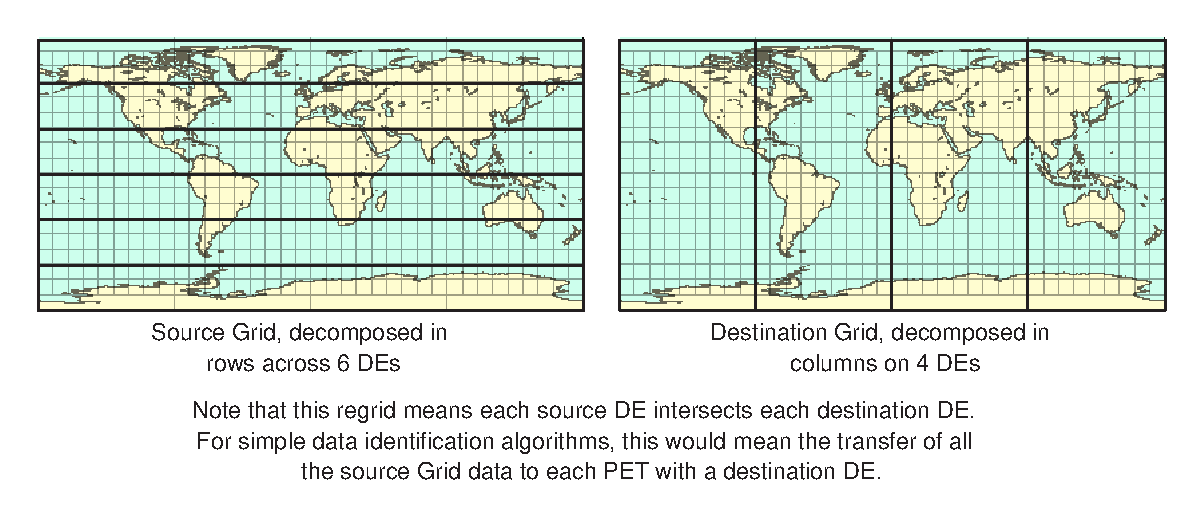
\includegraphics{RToCRegrid2002}
\end{figure}
\end{center}

still ultimately means copying all of the source Grid to each destination PET.
It often makes more sense to identify and transfer only the data from the
source Grid that is required by the destination DE.  In a parallel environment,
this means determining which source DEs intersect the local destination DE in
physical space, determining the extent of the data on that source DE that must
be transferred, and then gathering it to the local PET.  Both of these
approaches, either identifying the exact extent of the data that must be
communicated or communicating data as entire DEs, are currently implemented in
the framework.  By default the framework will transfer only the necessary data,
and the option is currently not readily available to users but is set internally
in the Grid code using a parameter called "domainOption."

This intersection of DEs is calculated in physical space, using a private Grid
method.  In complicated Grids, these intersections could be non-rectangular, but
for the current logically rectangular Grids each intersection is defined as the
block of the source DE that encompasses any physical overlap with the destination
DE's domain.  Future Grid types would need appropriate methods to identify
intersections, based on their topologies as well as communication issues.  As
shown in Figure \ref{fig:RegridIntersection}, 

\begin{center}
\begin{figure}
\caption{Intersection of DE Domains in Parallel Regridding. }
\label{fig:RegridIntersection}
\includegraphics{RegridIntersection2002}
\end{figure}
\end{center}

the intersection is often a subset of both the source and destination DEs'
domains, which means that each destination DE must receive and process data from
multiple source DEs.  Each PET involved in a regridding process must calculate
which other PETs it must send data to and how much (if it has a source DE) and
which it must receive data from and how much (if it has a destination DE).  The
current Grid structures contain enough global information to individually
determine the sending data, but the calculation of the data to be received takes
some global communication.

Regridding algorithms that are point-based (as opposed to cell-based), like
bilinear or bicubic interpolation, require an extra layer of cells around the
identified region, because those algorithms need the location of all surrounding
data points (see Figure \ref{fig:RegridExtraLayer}).

\begin{center}
\begin{figure} 
\caption{Illustration of the extra layer of points required by point-based Regrid
         algorithms. }
\label{fig:RegridExtraLayer}
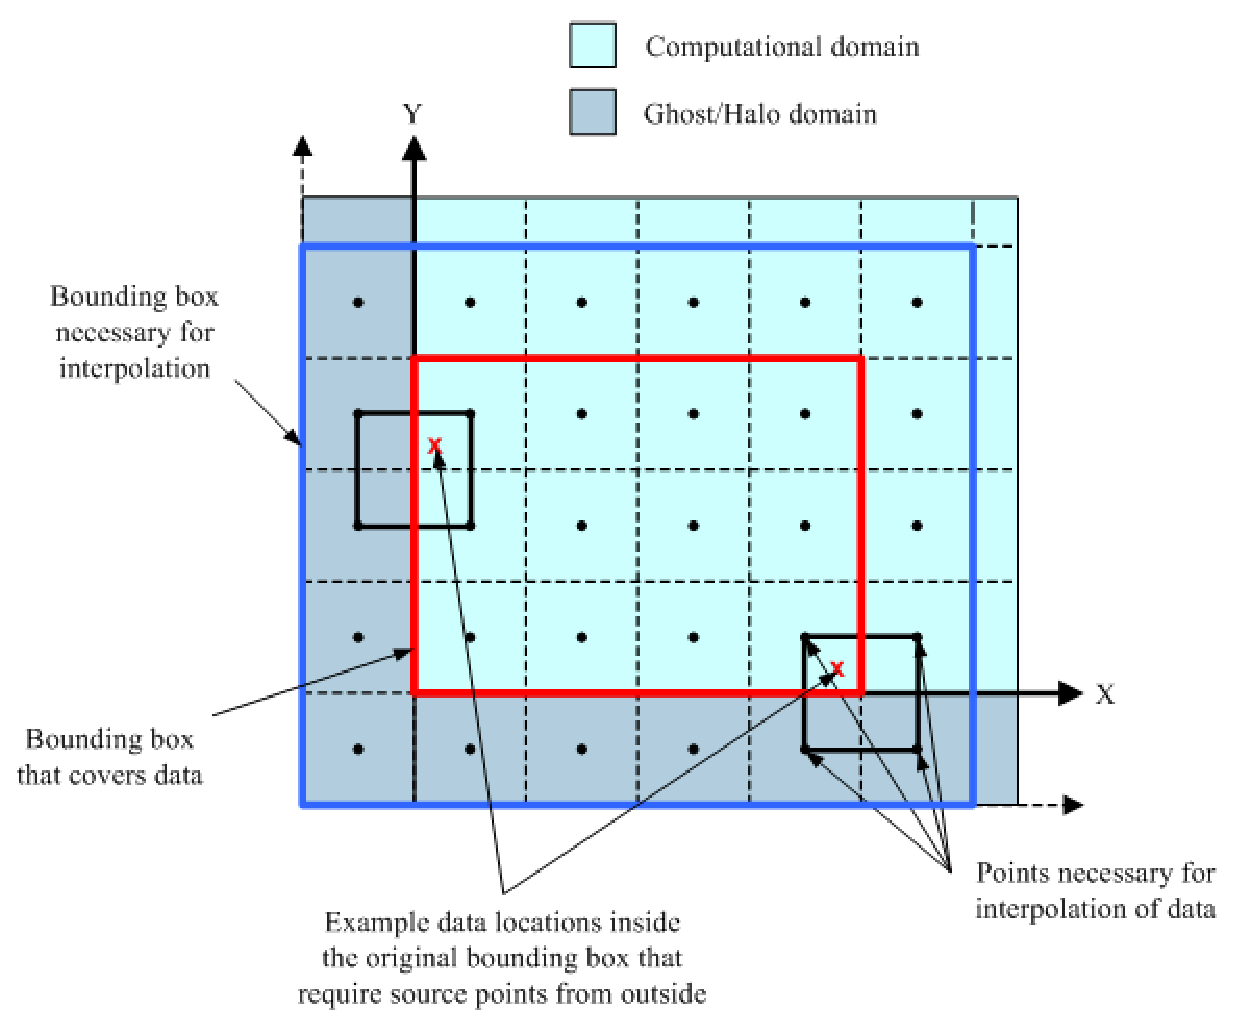
\includegraphics{RegridExtraLayer}
\end{figure}
\end{center}

Points in this extra layer are assigned internal mask values and are used in the
calculation of interpolation weights for data locations inside the identified
region, but are not assigned weights themselves.  However, these points could be
used in the future as a mechanism for regridding of periodic grids or to avoid
extrapolation issues near the edges of computational grids.

\subsubsection{Parallelization of Regrid: Data Transfer}
Once a block of data to send or receive has been identified, it is stored as an
internal structure called a {\tt domain} and added to a {\tt domainList}.  There
are separate send and receive domainLists for each DE.  From the domainLists,
all the sending and receiving information between PETs is stored internally as a
Route, so that it can leverage other ESMF code for efficient communication.
Internal to the Regrid Store routines, this Route is used to gather necessary
Grid coordinate information.  However, since Routes apply offsets in memory from
a base address rather than addresses themselves, these Routes are reusable by
structures that are distributed in the same way.  The Route to transfer Field
data is similar to that to move Grid coordinates but must be modified for any
Field ranks that do not correspond to a Grid axis and the Field's halo width and
lower bounds.   The modified Route is added to the RouteHandle that is returned
to users and applied later during the routine that actually regrids data from
one Field to another.

Each PET has its own unique Route.  The data it gathers, either Grid coordinates
or Field values, are stored locally as single 1D Arrays.


\subsubsection{Parallelization of Regrid: Sweep Algorithms}
The conservative regrid schemes create coordinate bins to decrease the
number of cells that must be swept, as described earlier.  SCRIP
had an input parameter to set the number of bins to be created, but for a
parallel implementation that number needs to be dynamic.  Dynamic binning
balances the cost, in terms of computational efficiency and storage, of setting
up bins with the savings of having fewer points in each bin to sweep through.  
Rather than specify a number of bins, ESMF added a parameter to set a targeted
number of cells per bin, called {\tt targetBinSize}.  The number of bins on any
PET is set by the local number of cells divided by the targetBinSize.  Currently
this parameter is hard-coded in Regrid, but could be made available to users.
It has been set to 250, based on some preliminary timings on its effect on
Regrid Store (see Figure \ref{fig:TargetBinSize}).

\begin{center}
\begin{figure}
\caption{Example of TargetBinSize on RegridStore timing. }
\label{fig:TargetBinSize}
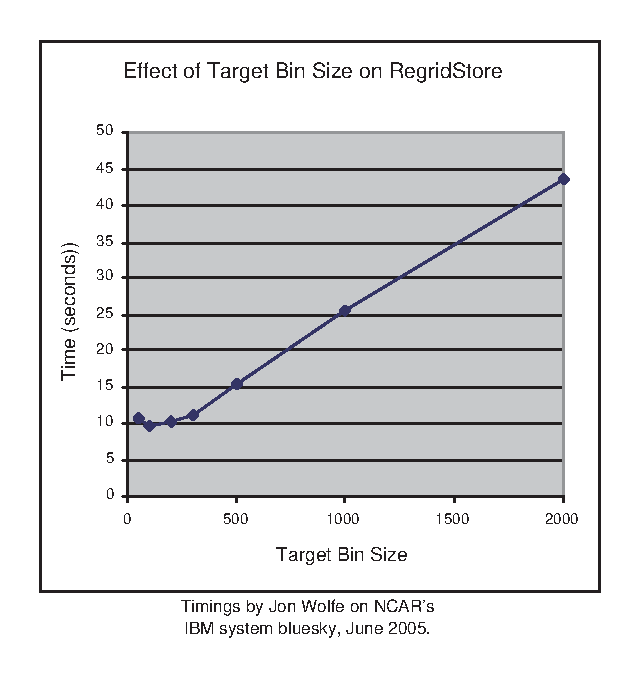
\includegraphics{TargetBinSize2002}
\end{figure}
\end{center}

Because the conservative regrid algorithm is based on cells and assumes data
values at the vertices, it can operate on the entire set of 1D Arrays of Grid
coordinate information at once.

The bilinear algorithm, on the other hand, is point-based and must assume the
data is logically rectangular.  For that reason, its sweep routine operates on
a single domain at a time, which typically represents just a part of the 1D
gathered Arrays.  It is otherwise unaffected by parallelization.


\subsubsection{Parallelization of Regrid: Calculation and Application of
               Interpolation Weights}

Once the necessary data has been identified and gathered, the calculation and
application of interpolation weights are entirely local operations, requiring no
inter-processor communication.  Once an interpolation weight has been determined
using one of the algorithms described earlier, the weight is stored as part of a
local list of links (described previously) in an object called an
{\tt ESMF\_TransformValues}.  This object is itself part of the 
{\tt ESMF\_RouteHandle} object, and contains:
\begin{description}
   \item [numlist]
         The number of links included in the object.  It also represents the
         size of the corresponding arrays.
   \item [srcindex]
         An array of indices into the local array of source data.
         This array is of size [numlist] and kind ESMF_KIND_I4.  Only a single
         integer is required to identify the source index because the source data
         has been gathered as a vector.
   \item [dstindex]
         An array of indices into the local array of destination data.
         This array is of size [2*numlist] and kind ESMF_KIND_I4.  Each
         destination index address requires two integers, one for each rank
         of the data array that corresponds to a Grid axis.  However, rather
         than being an array of rank 2, the index pairs are stored sequentially
         in the [dstindex] array.
   \item [weights]
         An array of interpolation weights.  This array is of size [numlist] and
         kind ESMF_KIND_R8.
\end{description}
Each link is represented by an entry in this set of arrays.  Also note that there
is a single link for each unique combination of source and destination indices.

The application of the interpolation weights occurs during the Regrid run
routines.  The only necessary communication is that to gather the required source
data locally into a one-dimensional array, using a precomputed Route.
Fundamentally, the application of the weights is a vector multiply of a sparse
matrix, with indirect addressing of the indices.  The main calculation is a loop
over the number of links that effectively sums the product of the source data and
the interpolation weights and loads the result into the corresponding destination
address.  A sample code fragment below illustrates the simplest case, where both
the source and destination data are two-dimensional arrays whose data axes 
correspond to the grids' exactly, with no reordering:

\begin{verbatim}
      do n = 1,numlinks     
        d1 = dstIndex((n-1)*2 + 1)
        d2 = dstIndex((n-1)*2 + 2) 
        s1 = srcIndex(n)           
        dstData2D(d1,d2) = dstData2D(d1,d2) &
                         + (gatheredData(s1) * weights(n))
      enddo  ! numlinks
\end{verbatim}

The coding becomes increasingly more complicated for data arrys of higher rank,
but is inherently similar.



\subsubsection{Regrid Objects}

There is no {\tt ESMF\_Regrid} object per se.  Users are returned an
{\tt ESMF_RouteHandle} object, which contains one or more {\tt ESMF\_Routes}
used to gather source data, an {\tt ESMF\_TransformValues} object with the
list of links, and an identifier for the type of RouteHandle.  All of these
objects are private and users are not expected to access or modify them.
